\chapter{Hardware}

Modern computers are a complex system of devices working together
to perform many tasks. A user will interact with a computer through
input and output devices (e.g. keyboards, mice, speakers, microphone,
and monitors).

\section{Computer Systems}

A computer systems is a collection of components that allows a user
to perform the basic operations of input processing, storage, control,
and output. Understanding how each of these components combine allows
us to create powerful information processing tools. Today we will talk
about each of these aspects in turn. Figure~\ref{fig:hardware:overview},
we see how some of these parts come together to form a computer system
(similar to the ones you'll use to program in this course).

\begin{figure}
	\centering
	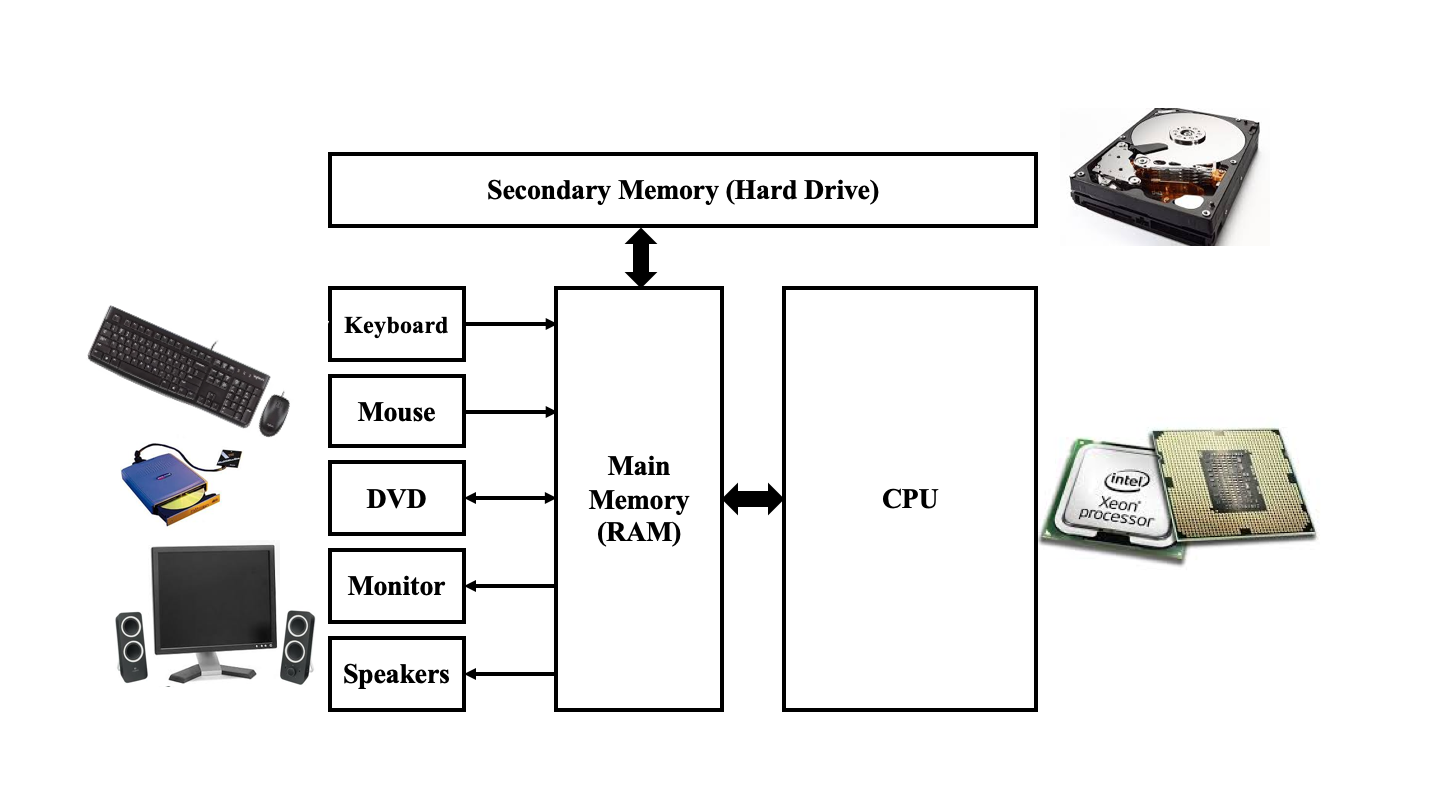
\includegraphics[width=0.5\textwidth]{images/cs_intro_hardware_overview.png}
	\caption{Interconnected parts of a computer system (keyboard, mouse,
                 monitor, DVD player / burner, speaker, hard drive, CPU).}
	\label{fig:hardware:overview}
\end{figure}

This lecture is meant to serve as an overview of several key parts of
computer systems. We'll focus on input and output devices, memory, and
the central processing unit (CPU) and how they work together.

\section{Input and Output Devices}

We'll begin with input and output devices. These are the parts of the
computer that we as users interact directly with. Without these devices,
we would be unable to interact with computer systems in any meaningful
way. The first computers would occupy a large room in an office building
and connect to a terminal (a keyboard and a text screen) in another room
for users to interact with. Thanks to Moore's Law, computers many orders
of magnituted more powerful can fit in the palm of your hand. Likewise,
the variety of input and output devices has multipled. We still have the
keyboard and monitor, we've added the mouse for interacting with graphical
displays. Today's phones are more computer than phone equipped with:
speakers, microphones, touch screens, cameras, fingerprint scanners, radio
transmitters, and much more. Computers even come embedded in other devices
like cars, traffic lights, X-ray machines, and thermostats to both control
and monitor the devices. As shown in Figure 1, these devices are generally
connected to a computer by connecting to the computer's memory. This is
called memory mapped IO (input and output). Input devices will write data
to a predefined location in memory in a known format and order. The
computer will then read the memory location and process the input as
desired. For output devices, the computer will write to the given memory
location allocated for the output device (again in an agreed upon format
and order) and the output device will the data and operate accordingly.

\begin{example}
Give Example Here (e.g. how monitors and keyboards work).
\end{example}

\section{Memory}

One of the most important parts of a computer, is the memory. There are two
major types of memory, Main Memory (RAM), and Secondary Memory (e.g. hard
disks, solid-state drives, tape drives, etc.) Main memory is voalitile,
meaning it only persists while the computer is on. Between turning a computer
on and off the main memory is whiped. Secondary memory, on the other hand
is persistent, it lasts between restarts of the computer system. Main memory,
is where the CPU stores programs and data it needs to execute instructions.
Secondary memory, is where persistent data such as files will be stored. When
the CPU needs, it can bring data from secondary storage to main memory or
persists data in main memory to secondary memory.

\section {Central Processing Unit}

The central processing unit (CPU) --- processor, main processor, etc. --- of a computer is the physical
circuitry of a computer that performs instructions. The CPU is in charge of fetching, decoding, and
executing all instructions. The basic building blocks of these instructions include arithmetic, logic,
control, input, and output. The set of basic instructions available to the CPU effects, what the computer
system can do (and how efficiently). Some CPU's are designed to handle a relatively small number of
instructions (integer addition, multiplication, division, conditional branching, store to memory, load
to memory). While others CPU's are designed to handle a large number of instructions (e.g. swap content
of memory locations, increment and store, etc. in addition to the simpler instructions).

While these instructions can be quite simple, we build up complex behaviours by combining these actions
into programs. When reasoning about how our programs will work, we should be aware of the limitations
imposed by the hardware we use. In mathematics, we often consider things in a very abstract way. In models
of computer systems, we often use unbounded arithmetic and allow a computer to have infinite memory; however,
in practice we need to run programs on processors with bounded computational and memory capabilities. In most
systems we encounter today, the CPU allows for 32 or 64 bit computations or memory read and writes in a single
instruction. Because reading and writing to memory takes a long time (in comparison to arithemetic and logic
instructions), almost all CPUs include a very small number of memory blocks on the physical CPU to store
intermediate results of instructions, called registers. In modern CPUs this is further increased by allowing
even more levels of memory, called caches (Level 1, Level 2, and Level 3), that trade off between speed of access
and the size of the memory. We won't go in depth on how these work, but briefly mention them to help you
understand how modern computer systems work to acheive greater efficiency.
